\chapter{Particle Reconstruction and Identification}
\label{ch:part_reco}

With a design luminosity of $1.0 \times 10^{34}$ cm\textsuperscript{-2}s\textsuperscript{-1}, and a peak Run-2 instantaneous luminosity of $2.0 \times 10^{34}$ cm\textsuperscript{-2}s\textsuperscript{-1}, reconstructing and identifying the products of LHC $pp$ collisions is one of the most complex tasks for each LHC experiment. The accurate reconstruction and identification of physics objects lays the ground work for all subsequent physics analyses, so it is also one of the most fundamentally important tasks performed by an experiment. \par

Reconstruction is the process of combining raw and uncalibrated hits across various subsystems into specific unique objects. Two particular subsystems, the Inner Detector (ID) tracker and the calorimeter play particularly important roles and will be discussed in detail. Analysis of the properties of the reconstructed objects identifies them as photon, electrons, muons, or jets. While photons, electrons, and muons are fundamental particles, jets represent a collimated shower of many hadronic particles, whose definition is more flexible. Jet reconstruction, clustering and substructure are all of particular important to jet identification, and to the later content of this thesis. Finally, reconstruction also identifies missing transverse energy \met in events, which is a crucial variable for BSM physics searches. Figure \ref{fig:detector_objects} shows how the various physics objects listed here interact with various systems in the ATLAS detector. 

\begin{figure}
        \centering
	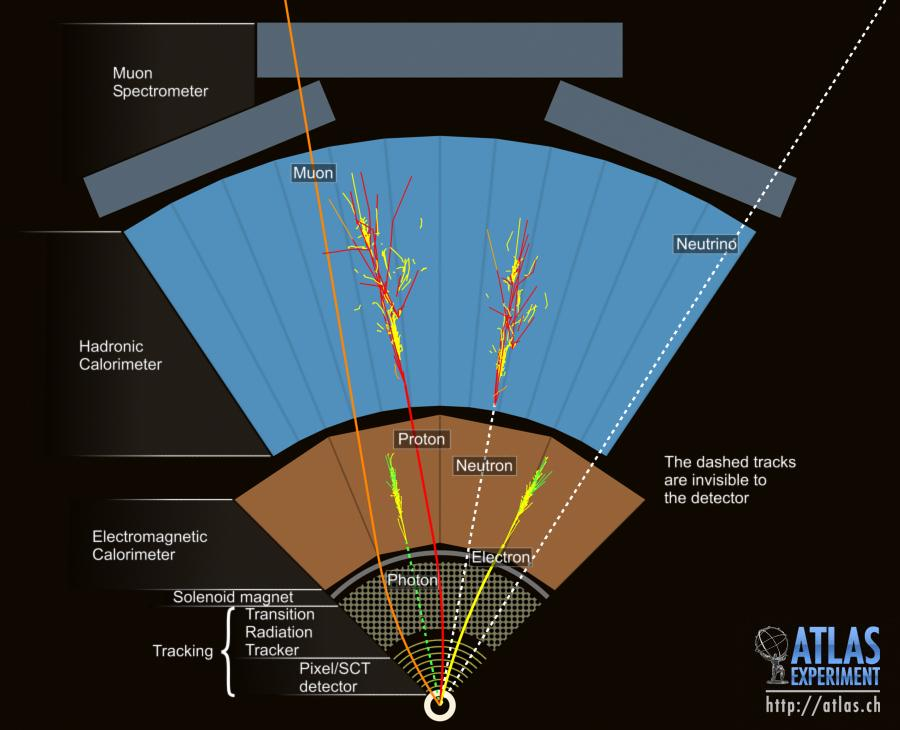
\includegraphics[width=0.8\textwidth]{figures/ch5/detector_objects}
	\caption{Graphic illustrating the various objects and high level features identified by ATLAS object reconstruction, and their interaction with different systems of the ATLAS detector \cite{detector_events}}
	\label{fig:detector_objects}
\end{figure}

\section{Inner Detector Tracks}
As the inner most layer of the detector, the ID measures charged particles close to the interaction point. The various hits of these charged particles throughout the ID are used to reconstruct \textit{tracks} which give the trajectories of charged particles. Track reconstruction begins by clustering hits in the Pixel and SCT detectors, and combining clusters from different radial laters of these detector. The multi-layer clusters form track \textit{seeds}, which provide initial estimates of measurements belonging to an individual track. The requirement of three points allows for a rough estimate of the track \pt to be made by calculating the curvature of the track and accounting of the magnetic field in the ID. \par

Tracks seeds are subject to a variety of quality requirements, such as having a minimum estimated \pt and passing interaction region compatability criterion. If these requirements are satisfied, the track seeds are passed to the track finding and fitting algorithms. The interplay of these three track reconstruction steps is illustrated in Figure \ref{fig:track_reco}. 

\begin{figure}
        \centering
	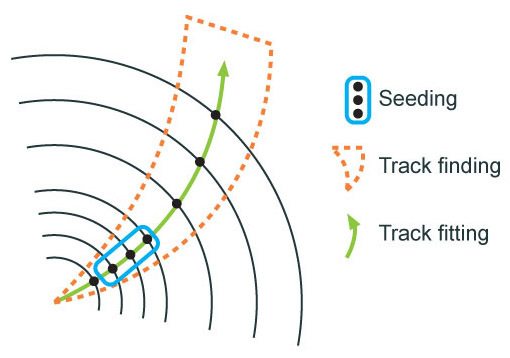
\includegraphics[width=0.6\textwidth]{figures/ch5/track_reco}
	\caption{Track reconstruction seeding, finding and fitting illustration \cite{track_finding}}
	\label{fig:track_reco}
\end{figure}


\section{Photons and Electrons}
\section{Muons}
\section{Jets}
\subsection{Calorimeter Clusters}
\subsection{Particle Flow Reconstruction}
\subsection{Jet Clustering}
\subsection{Jet Substructure}
\section{Missing Transverse Energy}
